
\chapter{Introduction}
\label{chap:intro}
%%%%%%%%%%%%%%%%%%%%%%%%%%%%%%%%%%%%%%%%%%%%%%%%%%%%%%%%%%%%%%%%%%%%%%%
%%%%%%%%%%%%%%%%%%%%%%%%%%%%%%%%%%%%%%%%%%%%%%%%%%%%%%%%%%%%%%%%%%%%%%%
%%%%%Overview%%%%%%%%%%%%%%
%%%%%%%%%%%%%%%%%%%%%%%%%%%%%%%%%%%%%%%%%%%%%%%%%%%%%%%%%%%%%%%%%%%%%%%
%%%%%%%%%%%%%%%%%%%%%%%%%%%%%%%%%%%%%%%%%%%%%%%%%%%%%%%%%%%%%%%%%%%%%%%

\section{Prelude}
\label{sec: overview}
%what doIhave inside galaxies:
% stuffIdon't care about because they don't have a big contribution on the SED 1) planets; 2) black holes 3) dark matter
Inside every galaxy, there are millions of stars, planets, and black holes, as well as dust and gas.
They all affect each others' formation, evolution, and extinction.
There is also dark matter inside every galaxy, which, to the best of our knowledge, only has gravitational effects on the other components.
Nearly all the information we can obtain from galaxies other than our own comes from their light.
Since each observable phenomenon inside galaxies emits most of its energy in specific wavelengths, 
a plot of brightness/flux density of galaxies as a function of wavelength, called a spectral energy distribution (SED), is a useful tool to understand galaxies. 
Young and evolved stars, dust, and gas in the space between the stars are the most important contributors to the spectral energy distributions of galaxies.
Planets and black holes without an accretion disc, on the other hand, have a much lower intensity compared to the other aforementioned components, and therefore contribute less to the SED.
Therefore, by properly modeling observed features in SEDs we can extract information about the evolution of stars, dust, and gas inside galaxies.

%stars
Arguably, stars are the main component of normal galaxies.
They control the chemical composition and structure of galaxies by transforming gas into new stars and by transforming dead stars back into gas.
They are also central to the formation and evolution of planetary systems.
The energy provided by stars is necessary to create and maintain the life on planets. 
The study of the formation and evolution of the Sun, and more generally that of stars, helps us understand more about our origin and the future of our Solar System.
Furthermore, in order to completely understand the formation and evolution of galaxies from the early universe to the current epoch, the knowledge of the formation and evolution of stars is necessary. 
As a result, the study of stellar formation and evolution has been a central topic in astronomy and astrophysics for decades.

%ISM 1)Gas 2)dust
%There could be a galaxy without stars (i.e. dark galaxies~\citep[][and references therein]{Cantalupo12}), but there will never be a galaxy without gas. %: this is a very strong statement. Some galaxies, like dwarf ellipticals, are pretty gas-free (at least now). So qualify this a bit. done
Among observable objects in galaxies, gas has a crucial role in formation and evolution of galaxies.
Gas and dust in galaxies can be found in the space between stars.
This space is called the interstellar medium (ISM), and is full of low density gaseous clouds with neutral or ionized atoms and/or molecules, and microscopic dust grains.
The gas and dust in the ISM are heated by interstellar radiation field and cooled through a variety of line and continuum processes which usually depend on the local physical conditions. 
The effect of the ISM on stellar formation is undeniable; it provides the raw material for the formation of stars~\citep[e.g.][]{Kennicutt08,Bigiel08}.
Studying the interstellar medium is not only essential to understanding the formation of stars, but is also  necessary for interpretation of stellar evolution due to fact that stars release their material into ISM when they reach the end of their evolutionary track.

In a galaxy like our own, star formation begins with the condensation of giant molecular clouds (GMCs, $\sim 10^7$ M$_{\odot}$) in the ISM due to gravitational instabilities. 
The denser regions within GMCs collapse under their own gravity (self-gravity) and create clumps.
Some of these clumps, which have a similar mass distribution to the stellar initial mass function (IMF), develop into self-gravitating cores.
Then these clumps continue to become denser and turn into protostars. 
Since the protostars have a higher mass than their surroundings, more gas from GMCs accretes onto protostars.
This procedure continues until hydrogen burning in centre of protostars starts (see~\cite{McKee07} for more detail). 

Metallicity, which is defined as the ratio of abundance of metals (any element heavier than hydrogen and helium) to the abundance of hydrogen, affects formation and evolution of stars indisputably.
\cite{Walch11} showed that in the case of large scale turbulence, the effect of metallicity on star formation is negligible, but if turbulence is decaying,  metallicity has a strong impact on stabilizing self-gravitating cores.
Metals also play an important role in heating, cooling, and ionizing processes in the ISM.
Since cooling is one of the main reasons for condensation of GMCs~\citep[e.g.][]{Maio07}, in low metallicity regions star formation may be suppressed. 
The amount of metals in stars affects their evolutionary tracks~\citep[e.g.][and references therein]{Maeder02}.
For instance, low metallicity stars tend to have lower mass loss via stellar winds than those with higher metallicity.
Observations show that massive low metallicity stars rotate faster.
Being more massive at the end of their evolutionary tracks gives massive low metallicity stars have a lower chance to explode and become a supernova.


%what does SED look like?
Our primary source of information about galaxies, specifically unresolved ones, is their spectral energy distributions. 
Broadly speaking, young and hot stars emit most of their light in ultraviolet (UV) wavelengths, evolved stellar populations show themselves in optical and near-infrared (NIR) emission, and gas and dust heated by stellar emission are bright in mid-infrared (MIR) or far-infrared (FIR) wavelengths.
Therefore, UV-to-IR SEDs contain valuable information about galaxies' stellar evolution and their ISM. 
Other wavelengths regimes in galaxy SEDs (e.g. X--ray, radio), that are dominated by processes such as active galactic nuclei, quasars, and supernovae shocks, are beyond the scope of this thesis.
The general shape of SEDs mirrors the morphological types of galaxies: starburst galaxies, which have high star formation rates (SFRs), emit the bulk of their energy in the UV, while the light of quiescent galaxies is dominated by optical and IR emission. 
Detailed information about the age of stellar populations and other properties of galaxies can be determined by modelling their SEDs.

 %how do you model it? %SED model CIGALE %Population synthesis ----> SFR, stellar mass 
The stellar population synthesis method, which sums stellar spectra to produce a composite spectrum, has been widely utilized since the 1970s~\citep[e.g.][]{Tinsley72,Searle73} to model SEDs of galaxies.
A thorough SED model must include stellar population models~\citep[e.g.][]{Bruzual93,Bruzual03,Maraston05}, stellar emission and dust attenuation~\citep[e.g.][]{Calzetti00,Dopita05}, dust grain emission such as from polycyclic aromatic hydrocarbons~\citep[PAHs; e.g.][and references therein]{Tielens08}, and IR emission from gas and dust~\citep[e.g.][]{Chary01,Dale02,Lagache03,Lagache04,Smith07a,Draine07}.
Many groups have modelled SEDs for different types of galaxies and created SED templates (for more information see the review of \cite{Walcher11} on fitting of SEDs and references therein).
Since the physical parameters of templates generated by the SED models are known, we can find properties of observed galaxies by fitting their SEDs (either by minimizing $\chi^2$ or by Bayesian analysis), using the templates.
One example of an SED-fitting code is {\em CIGALE}: Code Investigating GALaxy Emission~\citep{Noll09}.
It combines SED models and uses Bayesian analysis to find the best-fit SED for observed data in the rest-frame UV-to-IR.
Some of the physical properties of galaxies must be assumed as model input find the best SED, and others are derived from SED-fitting results~\citep[see][for more detail]{Walcher08}.
For example, the best-fit SED has information regarding star formation history and stellar mass to light ratio.
By integrating star formation history over a specific time scale, SFR can be derived.
Knowing the stellar mass to light ratio, one can use a galaxy's observed luminosity to calculate its stellar mass.

The formation of stars in galaxies depends on many parameters including gas mass, stellar mass, metallicity, dust, the galaxy's morphology, and the location of the star forming region inside the galaxy.
In extragalactic astronomy, measuring the rate at which stars form is uncertain and relies upon theoretical models and observational data.
Studying star formation and its relation to other quantities in galaxies is the subject of ongoing research.
In this chapter, I present a review of observational methods of measuring the star formation rate and the main properties that affect measuring and scaling the SFR. A discussion of the ISM and its role in star formation is presented in $\S$~\ref{sec: ism_intro}. In $\S$~\ref{sec: sfr_intro} I discuss measuring the star formation rate, followed by a discussion of the measurement of the stellar mass in $\S$~\ref{sec: starmass_intro}. Current issues about star formation and its relation to other properties of a galaxy are discussed in $\S$~\ref{sec: pre_intro}. 



%%%%%%%%%%%%%%%%%%%%%%%%%%%%%%%%%%%%%%%%%%%%%%%%%%%%%%%%%%%%%%%%%%%%%%%
%%%%%%%%%%%%%%%%%%%%%%%%%%%%%%%%%%%%%%%%%%%%%%%%%%%%%%%%%%%%%%%%%%%%%%%
%%%%%ISM%%%%%%%%%%%%%%
%%%%%%%%%%%%%%%%%%%%%%%%%%%%%%%%%%%%%%%%%%%%%%%%%%%%%%%%%%%%%%%%%%%%%%%
%%%%%%%%%%%%%%%%%%%%%%%%%%%%%%%%%%%%%%%%%%%%%%%%%%%%%%%%%%%%%%%%%%%%%%%


\section{Components of the Interstellar Medium} 
\label{sec: ism_intro}
%how do I observe it
%what the observation tell us
% how do I measure the dust and gas
The interstellar medium in galaxies is a complex system with a wide range of structures, but these structures can be divided into two main components: gas and dust.
The gas in the ISM of galaxies is mostly made of hydrogen and helium, with 1 per cent heavier elements (metals), and can be in the form of clouds or diffused regions.
Gas clouds include molecular clouds, cold neutral atomic hydrogen (\hi) or hot \hi~clouds, and diffuse gas can be either \hii~(ionized hydrogen) regions or a hot intercloud medium.
Dust is mostly comprised of silicates, and graphite grains can be seen in dark clouds or galactic cirrus.
Emission lines from atoms or ions (i.e \hii~regions) in a hot gas, lines from molecules in cold clouds, and 21~cm emission of \hi~are the main observational signatures of the gas in the ISM of galaxies.
Dust can be observed directly through far-infrared and sub-millimeter wavelength emission or indirectly through its extinction and attenuation effects (see Section~\ref{sec: extinction}).

Molecular clouds in the ISM are cold ($T \sim10$ K) and dense (particle number density $ 50<n<500$ cm$^{-3}$); masses of molecular clouds range from a few to millions of solar masses~\citep{Bolato08}.
Density in molecular clouds is not uniform. There are dense and cold clumps inside these clouds.
Since these clumps are ideal places to form stars, studying molecular clouds has an important role in understanding formation of stars.
However, H$_2$ molecules, the main component of molecular clouds, have no permanent electric dipole moment which makes them difficult to detect.
The second dominant component, helium, is a mono-atomic gas and has the same problem as hydrogen, but these clouds also contain heavier elements such as carbon monoxide, hydrogen cyanide, water, ammonia and more than tens of others.
Carbon monoxide (CO) molecules are the third-most abundant constituent of molecular clouds, and are easily observable.
Other heavier molecules have emission lines which are also detectable in the spectra of clouds (especially Galactic ones), but observing CO emission is the most common way to study the properties of molecular clouds i.e.\ their mass (see Section~\ref{sec: ismmap} for more details).

The molecular clouds are surrounded by clouds of atomic gas~\citep{Kennicutt12}, which are easily traceable by 21-cm emission.
Hydrogen atoms in the ISM (excluding the regions close to hot stars, see below) are in their ground state. 
The electron and proton spins in the ground state can be parallel (i.e. both spin up) or anti-parallel (i.e. the proton's spin is up and the electron's spin is down or vice versa). 
The energy of the anti-parallel mode is slightly less than the parallel mode.
Since atoms always want to be in the state with lowest energy possible, electrons in the parallel mode have a tendency to flip to the anti-parallel mode. 
However, the energy difference between these two states is very small and it takes millions of years before the transition happens.
The large amount of hydrogen atoms compensates for the rarity of the transition and at any given time, there are enough hydrogen atoms to emit the 21-cm radiation. 
Observation of the \hi~atoms is specifically necessary for understanding physical properties and dynamics of the ISM, which leads to understanding the star formation process~\citep{Walter08}.

\hii~regions are hot and low density regions that are mostly located in the disks of spiral galaxies.
High energy UV photons emitted by massive new born stars have sufficient energy to ionize their surrounding gas, and
~\halpha emission is the main observable feature of \hii~regions.
The temperature and density of these regions can be estimated by observing other recombination lines such as H$\beta$, and forbidden lines such as \sii, \oii, \oiii, and \nii. 
Forbidden lines are not called so because there is no chance of them occurring, but merely because their probability is much lower than the normal ``allowed'' transitions.
Optically bright \halpha emission from \hii~regions is correlated with number of new massive stars in regions, and can be used as a star formation tracer~\citep[e.g.][]{Kennicutt98b,Calzetti13}.
Studying \hii~regions provides valuable insight into star forming regions by providing information such as star formation rate, initial mass function (IMF), and distribution of ionizing stellar masses~\citep[][and references therein]{Azimlu11}.


Dust has an insignificant effect on the mass of the ISM, but it plays crucial roles in the ISM's evolution.
In spiral galaxies, dust grains are located in cold regions ($\sim$30~K) and have a power-law size distribution.
The source of energy for dust thermal emission is heating from stars, and the shape of the continuum depends on size of the grain.
Mid-infrared emission from dust grains is mainly dominated by PAHs heated by evolved stellar population~\cite{Smith07a} or recently formed intermediate-mass young stars~\citep{Peeters04}.
Large grains that are either heated by light from star-forming regions or by the interstellar radiation field from the total stellar population emit most of their light in far-infrared~\citep[e.g.][]{Calapa14, lu14}
Dust is the main source of extinction and reddening of starlight (see Sec.\ref{sec: extinction} for more information).

\subsection{Mapping the Interstellar Medium} 
\label{sec: ismmap}
Measuring the mass of gas in galaxies is a necessary step to knowing how much raw material is available for forming stars.
A map of the total gas mass in the ISM can be produced by direct observations of gas or using interstellar dust as a tracer. 
Neutral atomic and molecular hydrogen are the most common components of the ISM. 
Therefore, to produce a total gas mass map in galaxies, maps of these two components can be added together and multiplied by a constant factor to account for heavier elements (mostly helium) which cannot be observed directly. 
Another way to do the mapping is to assume that the ratio of total gas to dust is constant across the galaxy, and convert dust observations to a map of total gas mass.

\subsubsection{Direct Measurement of the Gas}

The surface density of gas in the ISM of galaxies can be measured by direct observation of the neutral and molecular hydrogen.
This method can be promising if observational data with resolved molecular and atomic clouds are available.
However, given the state of current technology, having high resolution images of clouds for most galaxies is not possible. 
This problem shows itself for distant galaxies more than nearby galaxies. 
As a result, using images of molecular and atomic gas clouds to measure surface density of gas in ISM is limited to the telescopes' resolution. 
 
%Most of our knowledge from molecular clouds comes from observing line emission of CO molecules, which {\bf due to their heavy weight, they have very low energy rotational state}(the state of angular momentum, J) and can be excited in the temperature of molecular clouds. %PB: need to fix text in {\bf} earlier in this sentence.
Most of our knowledge of molecular clouds come from observation of line emission of CO molecules, which, due to their large mass, possess a very low energy rotational state (the state of angular momentum, J) and can be excited in the temperature of molecular clouds. %Sr should I put the \bf back?
Given its low energy and critical density, CO can easily be excited even in cold molecular clouds.
Therefore, $^{12}$CO (usually the $J(1\rightarrow 0)$ rotational transition, observed at 2.6 mm) is used as a tracer of the mass of molecular clouds dominated by molecular hydrogen~\citep[e.g.][]{Sanders84}.
Higher rotational transitions of CO can be used as a tracer as well, but they are not as common as $J(1\rightarrow 0)$.

\cite{Young91} described the relationship between the CO luminosity of a cloud and its mass. The CO luminosity of a cloud is:
\begin{equation}
L_{CO} = D^2 \int I_{\rm CO} d\Omega, 
\end{equation}
%NOTE: Equations must be punctuated.%
where $D$ is the distance to the cloud and $I_{\mathrm CO}$ is the CO brightness temperature integrated over the line profile in K~km~s$^{-1}$.
It can be written as ${\int T_{\mathrm CO} dV}$ where $T_{\mathrm CO}$(K) is the peak brightness temperature in the CO line and $V$ is the line-width in km~s$^{-1}$.
For a uniform cloud with a radius $R$, the CO luminosity is given by:
 \begin{equation}
L_{\rm CO} = \pi R^2 T_{\rm CO} \Delta V.
\end{equation}

Giant molecular clouds are self-gravitating systems~\citep[e.g.][]{Efstathiou83,Blitz99}.
Thus, using the virial theorem leads to calculating the mass of the cloud: 
\begin{equation}
 \label{equ: vir}
 M_{cloud} = \frac{L_{\rm CO}}{T_{\rm CO}} \sqrt{\frac{4\rho}{3\pi G }},
\end{equation}
where $\rho$ is the mass density of the cloud and $\frac{1}{T_{\rm CO}}\sqrt{\frac{4\rho}{3\pi G}}$ is called the conversion factor.
Equ.~\ref{equ: vir} shows that the total mass of molecular clouds and the CO luminosity of the cloud are directly related~\citep{Young91}. 
Since the dependence of $I_{\mathrm CO}$ on optical depth is negligible~\citep{Krumholz09}, total CO luminosity can be used to measure the total H$_2$ mass of galaxies.
The relation between CO emission and H$_2$ cloud mass is shown to be
\begin{equation}
N_{\rm H_2}/\rm cm^{-2} = X_{\rm CO} \times I_{\rm CO}/{\rm K km s}^{-1},
\end{equation}
where X$_{\rm CO}$ is the conversion factor (also known as the X-factor).
The X-factor is different for each galaxy and sometimes is even different in regions within a galaxy due to differences in properties such as metallicity.
Although assuming a constant conversion factor for galaxies like M82 and M31 can lead to accurate estimation of global molecular gas mass, in regions with low metallicity this assumption leads to uncertainties~\citep{Bolato13}. 
Various groups are working on observations of different types of galaxies to measure the X-factor for them~\citep{Wilson95, Bosselli02, Bolato13}.


\begin{figure}
\centering
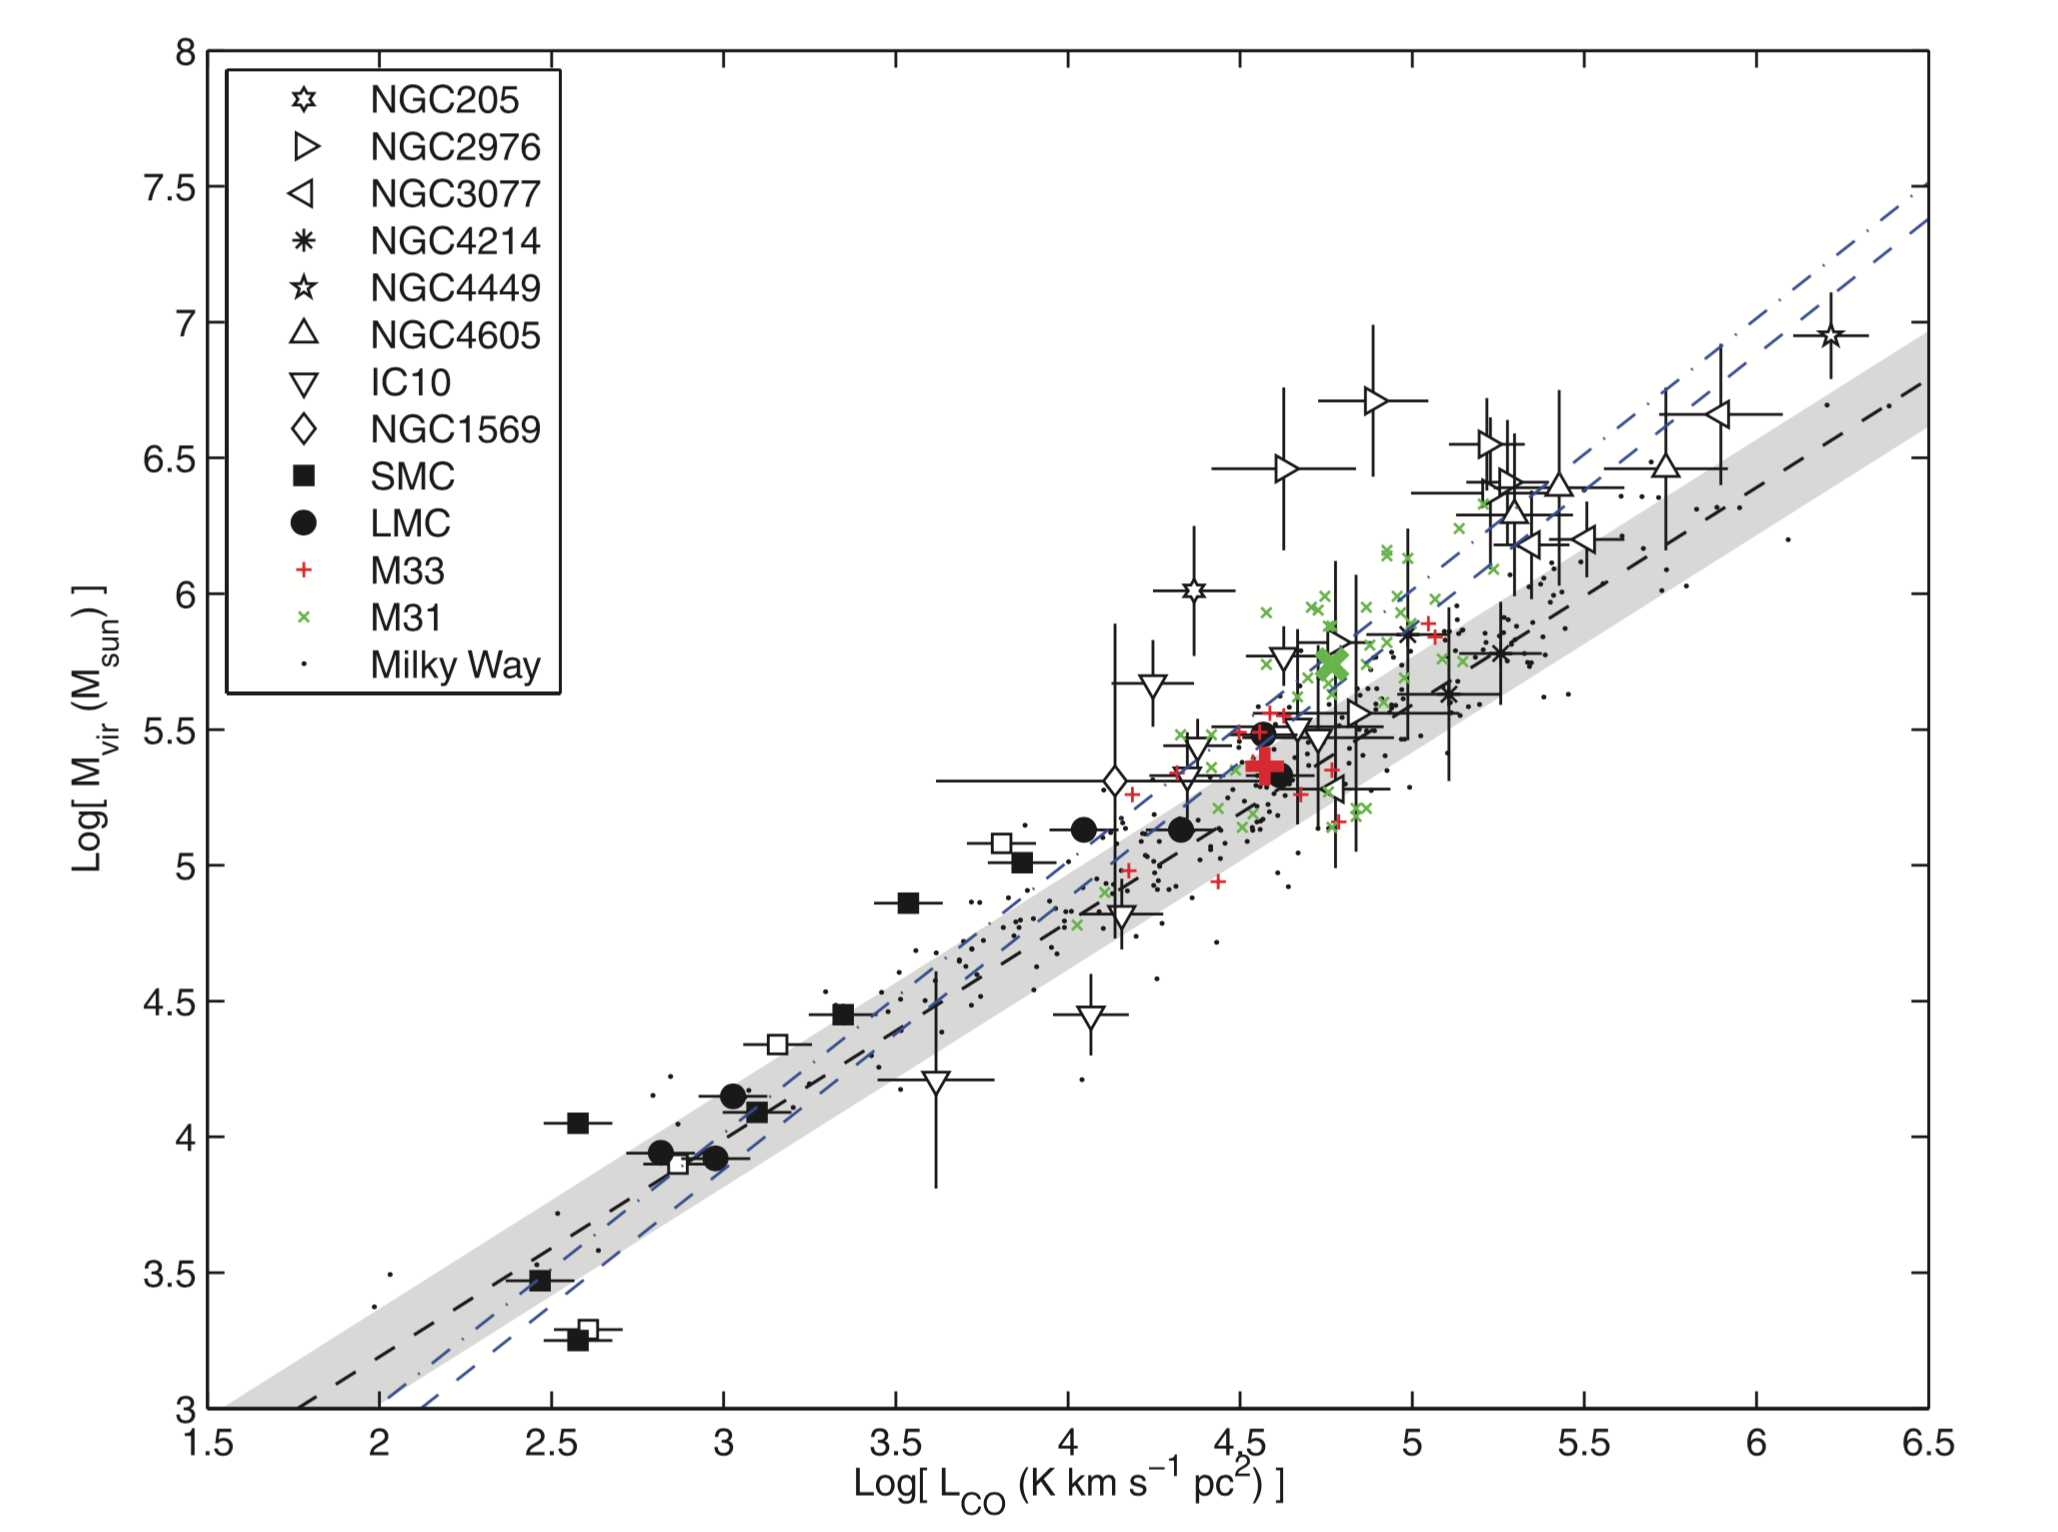
\includegraphics[width=\textwidth]{../image_intro/mvirial_lco.png}
\caption[Relation between the virial mass and CO luminosity]{Relation between the virial mass (M$_{\mathrm{vir}}$) and CO luminosity (L$_{\mathrm{CO}}$) for the Milky Way and extragalactic GMCs. The Milky Way data are shown by dots measured by~\cite{Solomon87}. Black and white symbols correspond to measurements based on $^{12}$CO~($J(2\rightarrow 1)$) and $^{12}$CO~($J(1\rightarrow 0)$), respectively. The black dashed line represents the Galactic mass-luminosity relation (M$_{\mathrm{vir}} \approx 39{\mathrm L}^{0.81}_{\mathrm{CO}}$) with gray region illustrating the Galactic 1$\sigma$ dispersion around the line.
The dot-dashed and blue dashed lines show the fits for dwarf sample and all extragalactic GMCs, respectively.
The extragalactic molecular clouds are very similar to those in the Milky Way. Adapted from~\cite{Bolato08}.}
\label{fig: mco}
\end{figure}

In order to empirically determine the relation between H$_2$ masses and CO luminosities, many observational attempts have been made on both Galactic and extragalactic scales. 
One of the most significant studies in this regard was done by~\cite{Solomon87}, who studied this relation over more than 273 clouds inside the Milky Way and found a strong correlation between the virial mass of molecular clouds and CO luminosity. 
In Local Group galaxies, several groups have measured size, line width, and CO luminosity of molecular clouds and investigated the relation between  their virial masses and CO emission in environments other than the Milky Way. 
Pioneering works in measuring the extragalactic conversion factor were done for M31 and M32~\citep[e.g.,][]{Wilson89, Wilson90}. 
Fig.~\ref{fig: mco} shows the CO luminosity versus virial masses of the Galactic and extragalactic molecular clouds. 
The extragalactic molecular clouds are similar to those in the Milky Way. 
The conversion between the CO luminosity and H$_2$ masses is still a controversial topic~\citep[e.g.][]{Narayanan11, Bolato13, Sandstrom13}.
Problems regarding metallicity are not yet resolved and it is still not clear whether the conversion factor is global or local. 
Extragalactic investigations have been limited to nearby galaxies due to telescope resolution and sensitivity. 
To measure the clouds in distant galaxies, the spatial resolution of maps must be better than 40~pc, which is the typical size of a giant molecular cloud~\citep[e.g.][and references therein]{Young91,Bolato13}. 

Atomic gas in galaxies is dominated by \hi~atoms, which are relatively easy to observe in 21-cm.
Assuming optically thin lines for \hi~emission, the intensity of the 21-cm emission is proportional to the density of the atomic hydrogen, $N_{H {\sc I}}$~(cm$^{-2}$), along the line-of-sight.
\begin{equation}
N_{H {\sc I}}  \propto \int T_{\mathrm B} dV
\end{equation}
where $T_{\mathrm B}$ is the temperature brightness in Kelvin and dV is in km~s$^{-1}$, with the integral over the line profile. 
These properties make the 21-cm line a very useful tool to study gas in the ISM and trace the large-scale distribution of galaxies in the universe (\hi~is detectable in most spiral galaxies and some elliptical galaxies).
Although the 21-cm emission is the most reliable technique to map the ISM, the linear relationship between the intensity and the column density of the gas breaks down when the gas is optically thick~\citep{Braun09}. 

\subsubsection{Dust Emission as a Tracer of Gas} 

Studying the gas clouds in the ISM of distant galaxies by using direct methods is almost impossible and not practical, due to low spatial resolution of available observational data.
\cite{Hildebran83} was the first to suggest that one way to estimate the mass of the gas in the ISM might be from the optical depth of the sub-mm continuum emission from the dust; continuum dust emission is generally optically thin. 
The Herschel Space Telescope~\citep{Pilbratt10} has measured the continuum dust emission from hundreds of galaxies~\citep{Eales10, Oliver12}. 
This amount of observational data provides a unique opportunity to study the ISM of galaxies using dust emission. 
The observed FIR flux has almost no dependency on distance, thus, one of the advantages of using the dust emission as a tracer of the gas mass is that unlike the direct method, high spatial resolution is not necessary. 
The other important advantage is that this method solves the newly-found problem of ``dark gas" in galaxies. 
Dark gas is a significant fraction of gas in galaxies which can be traced by neither the 21-cm emission nor the CO emission~\citep{Abdo10}. 
As such, it is very difficult to detect with telescopes, but an accurate gas to dust ratio can lead to an accurate estimate of dark gas mass in galaxies. 

There are disadvantages in using the gas to dust ratio to trace gas in the ISM.
In order to use the dust as a tracer of the gas mass, first a relationship between the optical depth and the mass of the dust and then a relationship between the mass of the dust and the mass of the gas must be derived.
\cite{Draine03} pointed out that the former approach is uncertain because of the uncertainly in the radiative efficiency of dust grains. 
Measuring the gas to dust ratio in galaxies are not accurate either~\citep{Hildebran83}, which means that there are problems in both steps. 
In addition, the dust method has two major practical problems: firstly, to apply this method, knowing the temperature of the dust is necessary. 
To solve this problem, measurement of the continuum emission at far-infrared wavelengths long enough to cover the peak of the emission must be very accurate~\citep{Ealas12}. 
The other problem is that there is evidence that the gas to dust ratio depends on the metallicity of the gas~\citep{Lisenfeld98, Draine07}, but even in direct methods the dependence on metallicity must be solved. 
Using dust emission as a tracer of gas is the best alternative for measuring the total gas in galaxies, that there is no observation of CO or \hi~emission. 

\subsection{The ISM and starlight: extinction and attenuation}
\label{sec: extinction}
Dust in ISM affects stellar emission by attenuating, scattering or absorption.
Effect of dust clouds with embedded light sources on distribution of the light is called attenuation. 
The dust cloud could have any distribution and be clumpy or smooth. 
Since both light source and dust have extended distributions, the relative locations of the dust and light source affect the net absorbed and scattered light.
The other parameter that is important for the scattering and absorption is the relative position of dust and observer.
When the dust is in the line of sight, attenuation will make the emerging light dimmer~\citep[e.g.][and references therein]{Calzetti13}.
This is the typically occurring situation when studying galaxies or extended regions within galaxies.

Extinction happens when there is a combination of both absorption and scattering of radiation by dust.
This effect grows inversely with wavelength.
%Extinction can be defined as a reduction of the original intensity caused by dust:
Extinction is quantified as the difference in observed and initial magnitudes of an object in a specific wavelength ($\lambda$):
\begin{equation}
m_{\lambda} - m_{\lambda}(0) = \mathrm{A}_{\lambda},
\end{equation}
where $\mathrm{A}_{\lambda}$ is the extinction, and $m_{\lambda}$ and $m_{\lambda}(0)$ are observed and initial magnitude, respectively.
Magnitude is related to intensity (I) as:
\begin{equation}
m_{\lambda} = 2.5 \log (I_{\lambda}) + C,
\end{equation}
where $c$ is a constant which depends on photometric system that is being used.
Optical depth, $\tau_{\lambda}$, is defined by ratio of observed and initial intensity of a source as:
\begin{equation}
\label{equ: extinction}
{\mathrm I}(\lambda) = {\mathrm I}_0(\lambda)\exp[-\tau_{\lambda}],
\end{equation}
where I$(\lambda)$ is observed intensity in wavelength $\lambda$ and I$_0(\lambda)$ is intensity of light before passing through dust.
Therefore, the optical depth and extinction can be converted to one an other by $\tau_{\lambda} = 1.086 \mathrm{A}_{\lambda}$. 
The extinction also depends on the grain size and extinction cross section.
For measuring SFR using various wavebands, decreasing of the intensity of radiation must be calculated and corrected for each wavelength; otherwise, there will be an underestimation of SFR. 

%%%%%%%%%%%%%%%%%%%%%%%%%%%%%%%%%%%%%%%%%%%%%%%%%%%%%%%%%%%%%%%%%%%%%%%
%%%%%%%%%%%%%%%%%%%%%%%%%%%%%%%%%%%%%%%%%%%%%%%%%%%%%%%%%%%%%%%%%%%%%%%
%%%%%SFR%%%%%%%%%%%%%%
%%%%%%%%%%%%%%%%%%%%%%%%%%%%%%%%%%%%%%%%%%%%%%%%%%%%%%%%%%%%%%%%%%%%%%%
%%%%%%%%%%%%%%%%%%%%%%%%%%%%%%%%%%%%%%%%%%%%%%%%%%%%%%%%%%%%%%%%%%%%%%%

\section{Measuring the star formation rate in galaxies} 
\label{sec: sfr_intro}
Understanding the formation of stars leads to better understanding of galaxies' formation and evolution. 
Characterisation of the star formation processes such as star formation rate (SFR) and the stellar initial mass function (IMF) is necessary in examining galaxies' structure formation~\citep{McKee07}. 
Measuring the SFR is not trivial and depends on a galaxy's morphology, metallicity, IMF, observational spatial resolution, and other properties. 
There is a large number of review papers on how stars form and how their formation is traced. 
From a theoretical perspective, one can refer to the classic picture of the theory of star formation as reviewed by \cite{Shu87} and more recently by~\cite{McKee07}. 
From an observational standpoint, star formation is discussed by many authers \citep[e.g.][and references therein]{Kennicutt98b, Kewley02, Calzetti13, Boquien10, Kennicutt12}.

In principle, emission from new stars can be traced by ultraviolet, visible light, near-IR and radio wavelengths, hydrogen recombination lines, forbidden metal lines, and also in the sub-mm range by using the Bremsstrahlung emission. 
Some of this emission is directly from stars, e.g.\ UV emission, and some is from ISM components that absorb and re-emit light from young stars, e.g.\ far-infrared emission.
Techniques to calibrate emission from newly-born stars, preferably hot and massive ones, to the rate at which stars are being formed have been the subject of many studies~\citep[e.g.][]{Calzetti07, Kennicutt11, Hao11,Bigiel08}. 
Peak of emission of young, hot, and massive stars is in UV wavelength, which makes them an ideal tracer of the current SFR.
One of the main assumptions in using the luminosity of massive stars is that the SFR has remained largely constant during the timescale probed by the specific wavelength which is being used as the tracer. 
By knowing the IMF, the number of massive stars can be used to extrapolate the total number of stars formed in a given star-forming region.
To have a reliable SFR indicator, the stellar IMF must be fully sampled to have at least one star in all mass bins (for more detail see Section~\ref{sec: imf}).
In general each tracer has some systematic errors, and one should decide which tracer is more accurate for a given system. 

\subsection{Stellar Initial Mass Function}
\label{sec: imf}
Stellar mass determines the important properties of a star, such as luminosity, lifetime and its evolutionary path. 
One of the most fundamental and difficult questions that a complete theory of star formation must answer is what is the stellar initial mass distribution of a star forming region.
Since most SFR calibrations use emission from stars in a specific mass range, it is necessary to know the stellar IMF to extrapolate to the full stellar population.
\cite{Salpeter55} empirically derived the stellar IMF from the observed stellar luminosity function of the Solar neighbourhood~\citep{Shu87}. 
He introduced a power-law IMF $\Phi$  in the form:
\begin{equation}
\label{equ: salp}
\Phi (\log M) = dN / d \log M \propto M^{-\gamma }
\end{equation} 
where $M$ is the stellar mass, $\gamma$ is a power-law index, and $N$ is the number of stars in the logarithmic mass range of $\log M$ to $\log M + d\log M$. 

In the late 1970s, it was recognised that the assumption of a the single power-law IMF over all stellar masses is not correct and might overestimate the number of low-mass stars~\citep{Kroupa93, Bastin10}. 
Since then, many groups have studied the stellar IMF and found different power-law relations (Fig.~\ref{fig: imf} ). 
Most SFR calibrations have the same assumption that the stellar IMF is constant across all environments and adopt it from the standard stellar IMF introduced by\ \cite{Kroupa01}:
\begin{equation}
\begin{split}
    \Phi (\log M) & \propto M^{-2.3}    \quad    (0.1 \le M(M{\odot}) \le 0.5)\\                  
           & \propto M^{-3.3}    \quad    (0.5 \le M(M{\odot}) \le 100)
\end{split}
\end{equation}
Although the Salpeter IMF produces more low-mass stars than the Kroupa IMF, they produce almost the same number of high-mass stars. 
Therefore, the SFR calibrations, which mostly trace massive stars in galaxies, based on the Kroupa IMF can be converted to the Salpeter IMF by multiplying the calibration constant by 0.67~\citep{Madau14}.
In a more recent study,~\cite{Weisz15} used data from the Panchromatic Hubble Andromeda Treasury program~\citep[PHAT][]{Dalcanton12} and showed that for nearby galaxies both Kroupa and Salpeter stellar IMFs overestimate the number of stars with masses greater than 8M$_\odot$.
\cite{Bastin10} reviewed the stellar IMF as derived from many observational results and showed that the stellar IMF is constant and universal, though there are uncertainties in different mass bins especially at the high-mass end. 

\begin{figure}
\centering
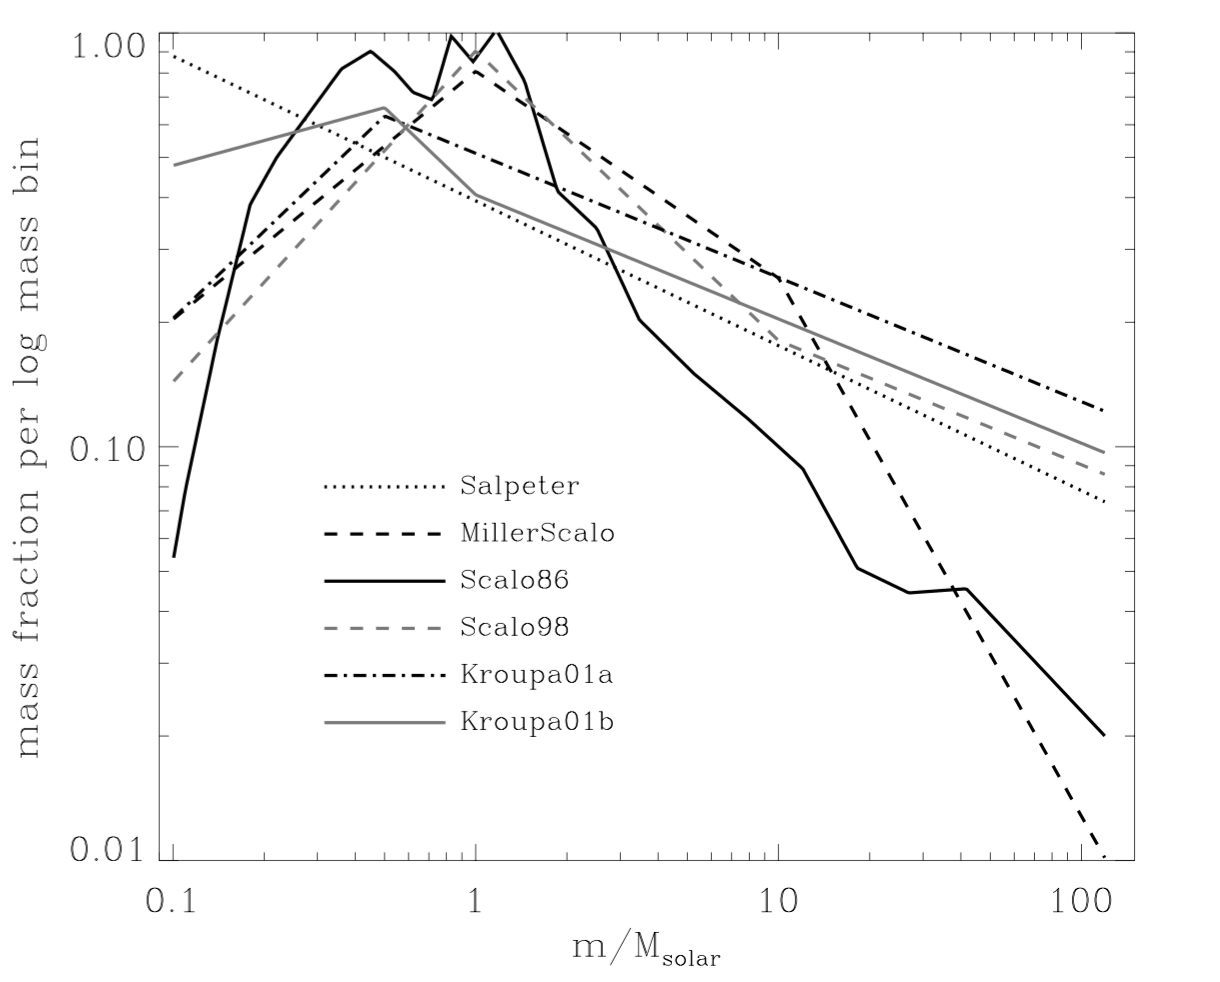
\includegraphics[width=16cm]{../image_intro/imf.png}
\small
\caption[Comparing stellar initial mass functions]{Comparing stellar initial mass functions (IMFs) by plotting the mass fraction per dex, power of 10, versus mass, normalized so that the integral under each curve is unity. The mass ranges from 0.1 to 120~M$_\odot$. Adopted from~\cite{Baldry03}.} 
\label{fig: imf}
\end{figure}


Since in using SFR calibration for different galaxies, I assume the initial mass function is universal, careful measurement of the IMF is the key factor in understanding the star formation rate. 
In distant galaxies, only massive stars can be detected; therefore, the IMF must be assumed to include all stellar mass ranges in the SFR calibrations. 
To show the impact of the different stellar IMF assumptions on the SFR calibrations, \cite{Calzetti13} used two different stellar IMFs and derived the SFR calibrations with these new assumptions.
Adopting a modified \cite{Kroupa01} IMF, with its maximum stellar mass set to 30~M$_{\odot}$ instead of 100~M$_{\odot}$, changes the SFR calibration constants by factors ranging from 1.4 to 5.6 for different SFR indicators (Table~\ref{table1}). 

\subsection{SFR Indicators}

One of the main issues in studying star formation in distant galaxies is the calibration of star formation rate indicators~\citep[e.g.,][]{Lee10}. 
Calibration of SFR indicators can be affected by differences in star formation history (SFH), metallicity, distribution of stellar population and dust in galaxies~\citep{Calzetti13}. 
Based on the spatial resolution of a system, one can divide star formation indicators into two categories: resolved and unresolved star formation indicators.

\subsubsection{Resolved Star Formation Indicators}
The most direct way to measure the SFR and trace recent star formation is counting individual objects~\citep{Kennicutt12}. 
These objects mostly few million years old and usually are referred to as young stellar objects (YSOs). 
Counting YSOs is used for calculating star formation rates in molecular clouds within $0.5- 1$~kpc of the Solar System. 
The number of YSOs can be converted to SFR using: 
\begin{equation}
SFR(YSO) = N_{yso} <M>/\tau 
\end{equation}
where SFR(YSO) is in units of M$_{\odot}$~yr$^{-1}$, N$_{yso}$ is the number of YSOs.
$<$M$>$ is the mean mass of YSO which depends on the IMF and considering current IMFs $<$M$> = $0.5~M$_{\odot}$ ~\citep[][]{Kennicutt12}. 
$\tau$ is the lifetime of the YSO  $\tau \sim 2$~Myr~\citep{Evans09}. 
Since our current devices cannot resolve individual YSOs, this method can only be applied to the Milky Way and its neighbourhood. 

In theory, for any system with high enough spatial resolution, counting YSOs can be used as a tracer of the star formation. 
However, considering the limited capabilities of the present instruments, YSOs in most regions beyond the Magellanic Clouds (satellite galaxies of the Milky Way at a distance of 0.05 Mpc) cannot be resolved. 
Therefore, most studies use the emission from the energetic young stars as a tracer of the SFR. 

%% and the continuation


\subsubsection{Unresolved Star Formation Indicators}

In star-forming regions farther away than the Magellanic Clouds, the spatial resolution of currently-available observations is not high enough to find all the young stellar objects. 
In unresolved systems, calibrating continuum or line emission at wavelengths sensitive to the young massive stars is the primary method of measuring SFR~\citep[e.g.,][]{Kennicutt98b, Kewley02, Bell03, Calzetti07, Calzetti08, Calzetti10, Calzetti13, Kennicutt07, Kennicutt09, Boquien10, Hao11, Kennicutt12}. 
\cite{Kennicutt98b} calibrated the luminosities of galaxies at specific wavelengths for measuring the SFR, using relations between the SFR per unit mass or per unit luminosity and the integrated colour of a system provided by stellar populations synthesis models~\citep[e.g.,][]{Bruzual93}. 

In unresolved systems, SFR indicators can be divided into local and global indicators. 
The global SFR indicators are defined for the entire galaxy; therefore, they are luminosity-weighted averages across local star formation history and the physical condition inside each galaxy. 
Local calibration is used for regions within a galaxy~\citep[e.g.,][]{Zhu08, Kennicutt09, Boquien10, Boquien11, Hao11}.
Limitations in the spatial resolution of observational data on the one hand, and the broader applicability to distant galaxy populations on the other, have in the past brought more attention to the calibrations of global SFR compared to local SFR. 
Because of its ability to trace the physical processes of the star formation, local SFR calibration is becoming increasingly important~\citep{Calzetti13}.

\subsubsection*{SFR Indicators Based on Single-Band Emission}

In order to derive conversions between the luminosity in specific wavelengths and the SFR, stellar population synthesis models are used~\citep{Kennicutt98b}. 
The general form of a SFR calibration using single-band emission is: 
\begin{equation}
\label{equ: sfrsingle}
{\rm SFR}(\lambda)= CL(\lambda),
\end{equation}
where SFR is in units of M${_\odot}$~yr$^{-1}$, $L(\lambda)$ is the luminosity in erg~s$^{-1}$ at the wavelength $\lambda$, and $C$ is a constant derived from stellar population models~\citep[e.g, starburst99][]{Leitherer99}). 
The constant $C$ varies for different wavelengths, mass ranges of the stellar IMF, and the timescale $\tau$ over which star formation is assumed to remain constant. 
Table~\ref{table1}, from \cite{Calzetti13}, summarises some values of $C$ and their changes according to different assumptions about the IMF. 


\begin{table}
\caption{Luminosity-to-SFR calibrations adapted from~\cite{Calzetti13}}
\label{table1}
\begin{center}
\begin{tabular}{ c c c }
\hline\hline
Luminosity$^1$ & C$^2$ & Assumptions$^3$\\
\hline
L$_{UV}$ & $3.0 \times 10^{(-47)} \lambda$ &$0.1 -100 M_{\odot}, \tau \ge 100 Myr $\\
L$_{UV}$ & $4.2 \times 10^{(-47)} \lambda$ &$0.1 -30 M_{\odot}, \tau \ge 100 Myr $\\
L$_{UV}$ & $4.3 \times 10^{(-47)}\lambda$ &$0.1 -100 M_{\odot}, \tau = 10 Myr $\\
L$_{UV}$ & $1.0 \times 10^{(-46)}\lambda$ &$0.1 -100 M_{\odot}, \tau = 100 Myr $\\
L(TIR) & $1.6 \times 10^{(-44)}$ &$0.1 -100 M_{\odot}, \tau = 100 Myr $\\
L(TIR) & $2.8 \times 10^{(-44)}$ &$0.1 -100 M_{\odot}, \tau = 100 Myr $\\
L(TIR) & $4.1 \times 10^{(-44)}$ &$0.1 -30 M_{\odot}, \tau = 100 Myr $\\
L(TIR) & $3.7 \times 10^{(-44)}$ &$0.1 -100 M_{\odot}, \tau = 100 Myr $\\
L(TIR) & $8.3 \times 10^{(-44)}$ &$0.1 -100 M_{\odot}, \tau = 100 Myr $\\
L(H${\alpha}$) & $5.5 \times 10^{(-42)}$&$0.1 -100 M_{\odot},  \tau \ge 6 Myr $\\
L(H${\alpha}$) & $3.1 \times 10^{(-41)}$&$0.1 -30 M_{\odot},  \tau \ge 10 Myr $\\
\hline
\end{tabular}
\end{center}
\begin{tablenotes}
\item $^1$ Luminosities (except for UV) are in erg~s$^{-1}$ and are given as $\nu L_{\nu}$.
\item $^2$ The constant $C$ appears in Equ.~\ref{equ: sfrsingle}. For SFR(UV), the numerical value is multiplied by the wavelength $\lambda$ in \AA to convert luminosity density to luminosity. 
\item $^3$ Assumptions for the mass range of the stellar IMF, using the expression derived by \cite{Kroupa01} (see Section~\ref{sec: imf}), and for the timescale $\tau$.
\end{tablenotes}
\end{table}


The most common single-band tracer of star formation rate is the ultraviolet.
As mentioned before, UV emission is an excellent tracer for the SFR.
Using a spectral energy distribution (SED) from Starburst99, with solar metallicity, and assuming a~\cite{Kroupa01} stellar IMF with the timescale of over 100 Myr, SFR can be measured as~\citep{Leitherer99}:
\begin{equation}
SFR(UV) = 3.0 \times 10^{-47}\lambda L_{\lambda}
\end{equation}
where SFR(UV) is in M$_{\odot}$~yr$^{-1}$, $\lambda$ can be in the range of $(912< \lambda < 3000~$\AA), and $L_{\lambda}$ is in erg s$^{-1}$\AA.
As shown in Table~\ref{table1}, with changes in the stellar ranges of the IMF, during timescales longer than 100 Myr, the calibration constant only decreases by a few per cent.
The calibration constants' changes for shorter timescales are more significant and 
the their accuracy is 15 per cent which can vary as a function of $\lambda$~\citep{Calzetti13}.
Ultraviolet light can easily be absorbed or scattered by interstellar dust. 
Therefore, using the UV emission as a tracer might lead to underestimation of the SFR if dust extinction corrections are not applied (\cite{Kennicutt12}; also see Section~\ref{sec: ism_intro}). 

Another single-band SFR indicator is the emission from hydrogen recombination lines. 
Ionizing photons emitted from young massive stars ionize the surrounding gas. Hydrogen recombination line emission, such as the Balmer series lines of H${\alpha}$ ($0.6563 \mu$m) and H${\beta}$ ($0.4861 \mu$m), which are located in the optical wavelength range, are among the most traditional SFR indicators~\citep{Kennicutt98a}. 
The relationship between the intensity of a hydrogen recombination line and the ionizing photon rate for a nebula is derived using quantum mechanics. 
The assumption is that the nebula must be optically thick to ionizing photons~\citep{Osterbrock06}.
Being optically thick means that almost all transitions more energetic than Ly${\alpha}$ absorb and re-emit via Ly${\alpha}$ and longer wavelengths.
This is why the H${\alpha}$ emission line strength is greater in optically thick environments. The relation between the SFR, the luminosity of the \halpha\ emission line, and the ionizing photon rate is~\citep[e.g.,][]{Osterbrock06, Kennicutt98b}:
\begin{align}
\label{equ: halpha}
SFR(H\alpha) = 5.5 \times 10^{-42}L(H\alpha) \\
                     = 7.4 \times 10^{-54}Q(H^{\circ})
\end{align}
where SFR(\halpha) is in M$_{\odot}$~yr$^{-1}$, L(\halpha) is in erg~s$^{-1}$, and Q(H$^{\circ}$) is the ionizing photon rate in units of s$^{-1}$.
The constant on the right-hand side of Equ.~\ref{equ: halpha} is the resulting coefficient for electron temperature T$_{\mathrm{e}}=10000$~K and density n$_{\mathrm{e}}=100$~cm$^{-3}$ which is typical in the \hii~regions.
Dust extinction (Section~\ref{sec: ism_intro}) is the most important source of systematic error in calculating the SFR from hydrogen recombination lines.
The effects of dust must be measured and \halpha\ observations must be corrected for extinction (e.g. by adding lumincity at 24~$\mu$m (L(24~$\mu$m)) to account for dust emission) or this could lead to underestimating the SFR~\citep{Kennicutt98b}.


Another nebular line used as a tracer of the SFR is \oii~$\lambda$3727~\AA. 
Although the luminosities of forbidden lines do not correlate with the ionizing atoms directly, their extinction has a correlation with the \halpha\ emission. 
As a result, \oii~luminosity can be used as a tracer of the SFR through \halpha\ luminosity. 
\cite{Gallagher89} calibrated the SFR based on the \oii~luminosity by using a sample of 75 galaxies. 
Another calibration for this luminosity was derived by \cite{Kennicutt92}. 
In his review on the SFR,~\citep{Kennicutt98b} averaged these calibrations and derived the following relation:
\begin{equation}
SFR([O\ II]) = 1.4 \times 10^{-41} L([O\ II])
\end{equation}  
where SFR(\oii) is in M$_{\odot}$~yr$^{-1}$ and L(\oii) is in erg~s$^{-1}$.
Although SFR(\oii) is not as accurate as the SFR(\halpha), it is one of major SFR indicators in high-redshift galaxies.
In these galaxies, the \halpha\ emission line is redshifted out of the optical band.
Consequently, calibration of the strongest emission feature in the blue (\oii) as an SFR indicator is very useful~\citep{Kennicutt98b}.


Since interstellar dust absorbs approximately half of the starlight and re-emits in the infrared, the infrared emission can be used to trace the SFR.
The IR luminosity of a system depends not only on the amount of embedded dust, but also on the heating rate provided by the stars. 
Since young stars heat the dust to higher mean temperatures than old stellar populations, to first order, the shape of the thermal IR SED depends on the starlight SED~\citep{Helou86}.
The fact that the heating rate provided by the young stellar population is higher than the old stellar population indicates that dust heated by the former is more luminous and consequently its SED peaks at shorter wavelengths (observationally $\approx 60~\mu$m) in comparison with dust heated by old or low-mass stars.
Therefore, infrared observations are able to detect the emission from the dust heated by young stellar populations, and can be used as an SFR indicator.  

Two empirical single-band infrared star formation rate indicators are the 24~$\mu$m and 70~$\mu$m bands.  
The use of these two bands depends on the type of the galaxy under study or the physical environment in different regions within the galaxy. 
Since the luminosity of a stellar population with constant star formation increases with time, the IR emission, which is used as a tracer of the emission of the stellar population, has different calibration constants in the case of a global (the entire galaxy SFR indicator) or a local indicator.
That is because the global case includes the integrated stellar population of a galaxy, while the other is calculated from regions with short star formation timescales such as \hii~regions, large star-forming complexes, etc.~\cite{Calzetti13}.
Table~\ref{table2} shows the constant $C$ from Equ.\ref{equ: sfrsingle} for 24~$\mu$m and 70~$\mu$m luminosities, for local (spatial scale $\sim500$~pc for 24~$\mu$m and $\lesssim 1$ kpc for 70~$\mu$m) and global cases. 
\begin{center}
\begin{table}
\caption{Infrared luminosity to star formation rate calibrations}
\label{table2}
\begin{tabular}{ c c c c }
\hline\hline
Luminosity$^1$ & $C$ & Assumptions & References\\ 
\hline
L(24)$^{0.885}_{local}$ & $1.31 \times 10^{-38}$ &$1.10\times 10^{40} \le L(24) \le 3.10\times 10^{44}$&  \cite{Calzetti07}   \\ 
L(24)$_{global}$ & $2.04 \times 10^{-43}$ &$ 4.10\times 10^{42} \le L(24)  \le 5.10\times 10^{43}$& \cite{Calzetti07} \\
L(70)$_{local}$ & $9.4 \times 10^{-44} $ &$5.10\times 10^{40} \le  L(70) \le 5.10\times 10^{43}$& \cite{Li12} \\
L(70)$_{global}$& $5.9 \times 10^{-44}$ &$L(70) \ge 1.4 \times 10^{42} $& \cite{Li10}\\
\hline
\end{tabular}
\begin{tablenotes}
\item $^1$ Luminosities are in the form of L($\lambda$) = $\lambda$ L$_{\lambda}$ in erg s$^{-1}$.
\end{tablenotes}
\end{table}  
\end{center}



\subsubsection*{SFR Indicators Based on Multi-Band Emission}

%%add PAHs here
Despite the usefulness of having single-band SFR tracers, in many cases the corrections due to dust effects and luminosity ranges increase the uncertainty in measurements.
Nowadays, thanks to large surveys, enormous amounts of data are available at different wavelengths for galaxies, which allows for combining the emission from different bands and finding new calibrations.
The conversion between SFR and luminosities in multiple bands mostly helps to avoid problems regarding dust extinction or attenuation (see~\ref{sec: ism_intro}). 
The simplest possible way to combine luminosities at different bands in order to convert them to SFR is through a linear relation, for which the correlation with the SFR is empirically derived~\citep{Kennicutt12}.

The emission from dust heated by young stars changes by the amount of high energy photons emitted toward the dust and by the properties of the dust such as the grain size.
Therefore, calibration of SFR varies for each of the single-band IR emissions.
Assuming that dust heating is dominated by emission from young stars, integrating over the full wavelength range of the infrared part of the spectrum reveals the total infrared (TIR) emission of the system, which can be used as an SFR indicator~\citep{Kennicutt98b}. 
 
TIR luminosity can be measured from the integrated infrared SED or a calibration of spatially-resolved infrared photometry introduced by~\cite{Draine07}. 
\cite{Boquien10} modified calibration of the total infrared luminosity as: 
\begin{equation}
L(\rm TIR) = 0.95L(PAH 8 \mu m) + 1.15L(24 \mu m) + L(70 \mu m) + L(160 \mu m),
\end{equation}
where $L = \nu L_{\nu}$ is the luminosity in erg~s$^{-1}$ at frequency $\nu$. 
\cite{Calzetti07} indicated that the star formation rate calibration for a stellar population undergoing constant star formation over $\tau=$100~Myr is:
\begin{equation}
\label{sfr_tot_IR}
SFR(\rm TIR) = 2.8 \times10^{-44}L(\rm TIR),
\end{equation}
where SFR(TIR) is in M${\odot}$~yr$^{-1}$, and L(TIR) is in erg~s$^{-1}$. 


In Sec~\ref{sec: overview} I mentioned that emission from PAHs in ISM can be used as an SFR indicator~\citep[e.g.][]{Peeters04}.
Most studies used emission in broad infrared bands, which contain PAHs, to calibrate SFR~\citep[e.g.][]{Calzetti07}, but SFR can be calibrated using only the PAH features.
\cite{Shipley16} calibrated SFR using observations from 105 star-forming galaxies with $z < 0.4$ as:
\begin{equation}
\log SFR = A + B \log L_{\mathrm{PAH}, \lambda},
\end{equation}
where $L_{\mathrm{PAH}, \lambda}$ is the luminosity of the PAH features at 6.2, 7.7, 11.3~$\mu$m or combinations thereof, in erg~s$^{-1}$.
Table~\ref{table_PAH} shows the constants for each $L_{\mathrm{PAH}, \lambda}$.
These calibrations underestimate the SFR for low-redshift galaxies with IR luminosity more than $10^{12}$~erg~s$^{-1}$.
\cite{Shipley16} showed that using the 7.7~$\mu$m feature in the calibration reduces the scatter and concluded that this wavelength provides the most robust SFR tracer.


\begin{table}
\caption{SFR calibrations from PAH luminosities; adopted from~\cite{Shipley16}}
\label{table_PAH}
\begin{center}
\begin{tabular}{ l c c}
\hline\hline
PAH Feature(s) & A & B\\
\hline
6.2 + 7.7 + 11.3 & $ -42.56 \pm 0.03 $ &  $1.00 \pm 0.03$ \\ 
6.2 & $ -40.06 \pm 0.09 $ &  $0.96 \pm 0.04$ \\ 
7.7 & $ -42.38 \pm 0.06 $ &  $1.00 \pm 0.03$ \\ 
11.3 & $ -44.14 \pm 0.08 $ &  $1.06 \pm 0.03$ \\ 
6.2 + 7.7 & $ -42.05 \pm 0.04 $ &  $0.99 \pm 0.03$ \\ 
6.2 + 11.3 & $ -42.52 \pm 0.05 $ &  $1.01 \pm 0.03$ \\ 
7.7 + 11.3 & $ -42.85 \pm 0.04 $ &  $1.01 \pm 0.03$ \\ 
\hline
\end{tabular}
\end{center}
\end{table}  


The most common use of combining luminosities to trace the SFR is the combination of total infrared measurements with both far- and near-ultraviolet observations, with the latter being more commonly used. 
This combination helps to avoid uncertainties from corrections for dust attenuation in far-UV (FUV) observations~\citep[e.g.][]{Hao11}. The calibration is:
\begin{equation}
L_{FUV}(\rm corr) = L_{FUV}(\rm obs) + \alpha L_{\rm TIR},
\end{equation}
where the luminosities are $L = \nu L_{\nu}$ in erg~s$^{-1}$, and the coefficient $\alpha$ depends on the bandpasses chosen for the UV and IR measurements. $\alpha$ is usually less than 1 because significant amounts of IR emission in many galaxies are from dust heated by older populations of stars~\citep{Kennicutt12}. The coefficient $\alpha$ is calibrated both theoretically, using evolutionary synthesis models, and empirically, by using measurements of dust corrected SFRs~\citep[e.g.][]{Hao11, Leroy08}. 

Another common method for using the multi-wavelength indicator for star formation is using H${\alpha}$ emission in combination with the 24~$\mu$m emission. 
This combination gives a more accurate dust-corrected estimate of the SFR~\citep{Kennicutt09}:
\begin{equation} 
\label{equ: halphaplus24}
SFR = 7.9 \times 10^{-42}[L(H{\alpha})_{\rm obs} + 0.020L(24 \mu m)]
\end{equation}
where L(H${\alpha}$)$_{\rm obs}$ is the observed H${\alpha}$ luminosity without correction for internal dust attenuation, given in the unit of erg~s$^{-1}$. 
L(24) is the 24~$\mu$m IR luminosity in erg~s$^{-1}$, and SFR is in M$_{\odot}$~yr$^{-1}$.


The IR emission in the other band can be used for correcting dust effect on UV or \halpha emission (see Table~\ref{table3}). 
The corrected emission then can be used as a SFR tracer.
These composite SFR indicators also have systematic uncertainties; yet, it seems that there is a good correlation between multi-band tracers and single-band tracers. 
Moreover, less uncertainty arises in this case than when using the single-band emission as a tracer~\citep{Kennicutt09}. 


\begin{table}
\caption{Multi-wavelength dust-corrected luminosities, adopted from~\cite{Kennicutt12}}
\label{table3}
\begin{center}
\begin{tabular}{ c}
\hline\hline
Combined luminosities$^1$ \\
\hline
L(FUV)$_{\rm corr}$=L(FUV)$_{\rm obs}$ + 0.46L(TIR)$^2$\\
L(FUV)$_{\rm corr}$=L(FUV)$_{\rm obs}$ + 3.89L(24~$\mu$m)$^2$\\
L(NUV)$_{\rm corr}$=L(NUV)$_{\rm obs}$ + 0.27L(TIR)$^2$\\
L(NUV)$_{\rm corr}$=L(NUV)$_{\rm obs}$ + 2.26L(24~$\mu$m)$^2$\\
L(\halpha)$_{\rm corr}$=L(\halpha)$_{\rm obs}$ + 0.0024L(TIR)$^3$\\
L(\halpha)$_{\rm corr}$=L(\halpha)$_{\rm obs}$ + 0.020L(24~$\mu$m)$^3$\\
\hline
\end{tabular}
\end{center}
\begin{tablenotes}
\item $^1$ Luminosities are in the form of L($\lambda$) = $\lambda$ L$_{\lambda}$ in erg~s$^{-1}$ 
\item $^2$ Calibrated by~\cite{Hao11}
\item $^3$ Calibrated by~\cite{Kennicutt09}
\end{tablenotes}
\end{table}  


As mentioned in Section~\ref{sec: imf}, using different IMFs results in having different calibration constants for star formation rate. 
From Table~\ref{table1} it is clear that changing the IMF affects the H${\alpha}$ SFR calibration more than other SFR calibrations. 
This effect is more than four times larger than for UV SFR calibrations because newly-formed stars having up to $\sim 5$ M$_{\odot}$ emit more strongly at UV wavelengths than any other part of the spectrum; however, significant amounts of ionising photons are produced by stars more massive than $\sim 20$ M$_{\odot}$.
Furthermore, reaching an asymptotic value of ionizing photons takes longer for more massive stars (10 Myr for the upper mass limit of 30 M$_{\odot}$ versus 6 Myr for 100 M$_{\odot}$). 
Therefore, changes in the H${\alpha}$ SFR calibration constant are more pronounced, while for UV and TIR the calibration constants are fairly close to each other.
On the other hand, using the mean stellar mass for the Kroupa IMF $(<$M$> \sim 0.6$ M$_{\odot})$ yields less than a 10\% difference between using the upper mass limit of 100 M$_{\odot}$ and 30 M$_{\odot}$. 
As a result, calibrations derived with the mean stellar mass of a system are more accurate than those that are based on tracing the most massive stars~\citep{Calzetti13}.

Our understanding of star formation in extragalactic systems depends on the light emitted by those systems.
While emissions from massive and young stars are the dominating light of the system, mass of low-mass stars dominates the mass of the regions (see Section~\ref{sec: imf}).
Therefore, SFRs are calibrated based on the dominant light of the systems and low-mass stars are accounted for using the initial mass function.
Emission from star forming regions should be corrected before it can be used in calibrations.
On its way to the Earth this emission passes through dust and gas clouds which cause extinction or attenuation (see ref.~\ref{sec: extinction}).
On the other hand, evolved stars emit their light in the whole spectrum as well as the  UV. 
Therefore, even though it might have an insignificant part in UV emission from galaxies, a correction for emission from evolved stars should be considered~\citep{Leroy08}.
After measuring the corrected luminosities for star forming regions in galaxies (global or local), using proper calibrations can give the best estimation of SFR in galaxies. 




%%%%%%%%%%%%%%%%%%%%%%%%%%%%%%%%%%%%%%%%%%%%%%%%%%%%%%%%%%%%%%%%%%%%%%%
%%%%%%%%%%%%%%%%%%%%%%%%%%%%%%%%%%%%%%%%%%%%%%%%%%%%%%%%%%%%%%%%%%%%%%%
%%%%%Stellar Mass%%%%%%%%%%%%%%
%%%%%%%%%%%%%%%%%%%%%%%%%%%%%%%%%%%%%%%%%%%%%%%%%%%%%%%%%%%%%%%%%%%%%%%
%%%%%%%%%%%%%%%%%%%%%%%%%%%%%%%%%%%%%%%%%%%%%%%%%%%%%%%%%%%%%%%%%%%%%%%

\section{Stellar mass}
\label{sec: starmass_intro}
One of the most fundamental physical parameters that describes the present state of a galaxy is its stellar mass. 
Stellar mass is linked to the structure and star formation history of disc galaxies~\citep{Gavvazi96} and  galaxies of all morphologies~\citep{Scodeggio02}. 
Measuring the mass of a stellar population is indirect and subject to significant uncertainties. 
In principle there are two ways to measure stellar mass in galaxies. 
The first is measuring the dynamical mass of a galaxy using kinematics (the motion of stars)~\citep{Cappellari06} or gravitational lensing (the bending of light as it passes near a galaxy)~\citep{Auger09}, and then modeling the mass of the dark matter and subtracting it from the measured mass. 
The second method is based on stellar population models~\citep[e.g.][]{Bruzual93, Kotulla09} and using them to connect stellar mass to an observable, such as luminosity in different wavelengths, colours, or spectral energy distribution. 
Stellar population models predict the expected SEDs for stellar populations based on the parameters of the regions such as star formation history, metallicity, and IMF.
Uncertainties come from the uncertainties in the stellar initial mass function (see Section~\ref{sec: imf}), the stellar evolution models (especially the stage where stars have the most luminosity in their evolution), the evolutionary state of the galaxy~\citep[see][and references therein]{Dalcanton12}, and star formation histories. 


In order to translate between photometry and stellar mass, the stellar mass-to-light ratio ($M/L$) is needed.
The use of $M/L$ is one way to measure the stellar mass surface density. 
It is an indirect method and has high uncertainties in specific cases, but can help in studying the stellar mass in large samples. 
For integrated galaxy light, the $M/L$ is estimated using scaling relations between $M/L$ and broadband colours \citep[e.g.][]{Bell03}, and then multiplying this ratio by luminosity to estimate the mass.
For resolved galaxies, one can produce a map of the stellar mass surface density distribution in galaxies using resolved colours to measure spatial variations in $M/L$.
This method gives more accurate results than measuring the stellar mass surface density distribution from single-band images that are rescaled by a uniform mass to light ratio~\citep{Zibetti09}.

Comparing results from independent methods to measure stellar mass helps to determine whether there are any systematic differences.
Comparing the results from measuring stellar mass within galaxies shows that the differences are on the order of a few tens per cent~\citep{McLaughlin05}.
Therefore, to model subtleties, the advantages and disadvantages of using each method should be carefully considered. 


\subsection{Galaxy masses from dynamics}

The simplest and the most common way to estimate the mass of a galaxy is to assume that the dynamics of the galaxy are governed by simple Newtonian classical physics.
In this model, the circular velocity $v_{\mathrm{circ}}(r)$ of an orbit with radius $r$ within a spherical system of gravitational potential $\phi$ and mass $M$ is given by:
\begin{equation}
\label{eq: simpmass}
v^2_{\mathrm{circ}}(r)=r\frac{d\phi}{dr} = G\frac{M(r)}{r},
\end{equation}
where $G$ is the gravitational constant and $M(r)$ is the total mass within a sphere of radius $r$. 
For a flattened disk, which is the case in most spiral galaxies, the right hand side of Equ.\ref{eq: simpmass} is replaced by the more exact expression derived by~\cite{Freeman70}. 
For the case of no dark matter or bulge, \cite{Freeman70} showed that the rotation curve of a self-gravitating disk is:
\begin{equation}
v^2_{\mathrm{circ}}(R)= 4\pi G \Sigma_{0}R_{d} y^2[I_0(y)K_0(y) - I_1(y)K_1(y)],
\end{equation}
where $R$ is the distance from the centre, $\Sigma_0$ the central surface brightness, $R_d$ is the disk scale length where the ratio of the intensity of disk to bulge is equal to $e$.
$y$ is equal to $\frac{R}{2R_d}$, and $I_i(y)$ and $K_i(y)$ are  modified Bessel functions of the first and second kinds. 


The mass distribution in disk galaxies is usually calculated from rotation curves or integrated line profiles from emission lines such as H${\alpha}$, CO, or \hi. 
Integrated line widths only yield an estimate of total mass within some (uncertain) isophotal radius.
Thanks to the current generation of detectors, it is now possible to obtain very high-resolution spectra in the \halpha and CO lines over the most of the optical disks of galaxies.

A detailed description of calculating dynamical masses in galaxies is beyond the scope of this work. 
The methods mentioned here represent the first order of approximation. 
For more accurate results, one should consider non-circular rotational velocities and the fact that galaxies contain millions of stars plus interstellar objects; therefore simple two-object Newtonian physics is not sufficient. 
A detailed review of dynamical masses of galaxies can be found in \citet{Courteau13}.

\subsection{Galaxy masses from stellar population modelling}

Galaxies can be observed because of their stellar emission; stars radiate the energy produced from nuclear reactions in their cores. 
Given a star's initial mass, the theory of stellar evolution can describe the amount of released energy. 
Hence, stellar mass that is responsible for radiation of stars can be derived by modelling the spectral energy distributions of galaxies. 
However, some fraction of the mass of galaxies consist of evolved stars which no longer emit radiation yet still contribute to the galaxy mass as stellar remnants and should be considered in the models.
Stellar population synthesis models are used to predict the SED of a stellar population using many physical parameters. 
Some of these parameters, which control the time evolution of the stellar population, are age ($t$) of the population measured in years (also referred to as the time passed since the star formation began), IMF, and metallicity~\citep{Courteau13}.

The basic idea behind finding a suitable calibration between flux/luminosity of the stars in different wavelengths and stellar mass is that one can use the SFHs recovered from synthesizing the stellar optical colour-magnitude diagrams in different regions of a galaxy. 
The calculated stellar mass in nearby galaxies can be used to calibrate the fluxes from the stars in other galaxies.
\cite{Zibetti09} suggested that to reach the maximum spatial resolution one can recombine the photometric information on a pixel-by-pixel basis. 
They used this method to study the stellar mass distribution in galaxies as well as the dependence of the SED on stellar mass density.
To do so the surface density of stellar mass at each position is derived by 
\begin{equation}
\label{equ: massphot}
\Sigma_{{\mathrm M_\star}} (\alpha, \delta) = \Sigma_{\lambda}(\alpha, \delta) \gamma_{\lambda}(\alpha, \delta),
\end{equation}
where $\alpha$ and $\delta$ are sky position (right ascension and declination, respectively).
$\Sigma_{{\mathrm M_\star}} (\alpha, \delta)$ is the stellar surface density.
$\Sigma_{\lambda}(\alpha, \delta)$ is the surface brightness and $\gamma_{\lambda}(\alpha, \delta)$ is the effective stellar $M/L$ at an effective wavelength $\lambda$.
In Equ.\ref{equ: massphot},  $\gamma_{\lambda}$ can be described as a function of one or more colours as observed at the specified location in galaxy. 

The peak of emission from evolved stars is in the near-infrared part of the spectrum.
Therefore, many studies have tried to make a map of stellar mass distribution using this bandpass within galaxies~\citep[e.g.,][]{Elmgreen84}.
Thanks to the \Spitzer~\citep{Wener04} and WISE~\citep{Wright10} space telescopes, a large amount of data in these bands from many regions in the sky is available, which helps to give a more accurate calibration. 
Fluxes from 3.6 and 4.5~$\mu$m are suitable for calibration of the stellar mass, due to fact that these two band-passes not only trace evolved stellar population but are also almost insensitive to the emission from young stellar population and to dust absorption and emission. 
\cite{Zhu10} used the Sloan Digital Sky Survey~\citep[SDSS][]{York00} and the \Spitzer Wide-area Infrared Extragalactic Survey~\citep[SWIRE;][]{Lonsdale03} to find a calibration between galaxy luminosity and stellar mass. 
Using the $M/L$ of galaxies, they found correlations between $K_s$ band (2.2~$\mu$m), 3.6 and 4.5~$\mu$m band luminosities and stellar masses and formulated these correlations as:
\begin{equation}
\begin{split}
\label{equ: zhu1}
\log M_{\star} =& -1.60  + 1.12  \log \nu L_{\nu}[K_s]\\
\log M_{\star} =& -0.79 + 1.19 \log \nu L_{\nu}[3.6\mu \rm m]\\
\log M_{\star} =&-0.25 + 1.15\log \nu L_{\nu}[4.5\mu \rm m], 
\end{split}
\end{equation}
where M$_{\star}$ is the stellar mass in solar masses and $ \nu L_{\nu}[\lambda]$ is the luminosity in erg~s$^{-1}$ at a specified wavelength.

\cite{Eskew12} tested the 3.6- and 4.5 $\mu$m fluxes as proxies for stellar mass in the Large Magellanic Cloud and found an empirical relation between mass of the stars and the luminosities of stars as:
\begin{equation}
\label{equ:eskew}
  M_{\star} = 31.84 \times 10^{5.65} L_{3.6}^{2.85} L_{4.5}^{-1.85},
\end{equation}
where M$_{\star}$ is the stellar mass in solar masses, and $L = \nu L_{\nu}$ is luminosity in erg~s$^{-1}$~\AA$^{-1}$.
Equ.s in~\ref{equ: zhu1} were derived from a large sample of galaxies and tested on different types of regions and galaxies.
On the other hand,~\cite{Eskew12} mentioned that since their calibration is based on data from the Magellanic Clouds,
measuring the stellar mass from Equ.~\ref{equ:eskew} might break down for highly star-forming regions; moreover, this equation has not been tested on regions with different metallicities. 
%In more recent work,~\cite{Laura16} measured stellar mass for a group of galaxies with ($z < 0.035$) using correlation introduced by~\cite{Eskew12} and showed these stellar masses are tightly correlated with stellar masses measured from other calibrations.
In more recent work,~\cite{Laura16} measured stellar mass for a group of galaxies with $z < 0.035$, using the correlation that was introduced by~\cite{Eskew12}. 
The study revealed that measured stellar masses in that study are tightly correlated with stellar masses measured from other calibrations.
%%%%%%%%%%%%%%%%%%%%%%%%%%%%%%%%%%%%%%%%%%%%%%%%%%%%%%%%%%%%%%%%%%%%%%%
%%%%%%%%%%%%%%%%%%%%%%%%%%%%%%%%%%%%%%%%%%%%%%%%%%%%%%%%%%%%%%%%%%%%%%%
%%%%%Preview%%%%%%%%%%%%%%
%%%%%%%%%%%%%%%%%%%%%%%%%%%%%%%%%%%%%%%%%%%%%%%%%%%%%%%%%%%%%%%%%%%%%%%
%%%%%%%%%%%%%%%%%%%%%%%%%%%%%%%%%%%%%%%%%%%%%%%%%%%%%%%%%%%%%%%%%%%%%%%

\section{Preview}
\label{sec: pre_intro}

A complete picture of how galaxies are formed and evolve is tied to unfolding the mystery of the formation of stars.
Various phenomena affect the collapse of molecular clouds and star formation, including the environment of the star-forming region, chemical composition of the region, the initial density distribution of the gas and the mass of stars in galaxies.
For decades, observational, theoretical, and numerical studies have investigated star formation; nevertheless, their results are not in agreement.
Empirical studies are used alongside theoretical ones to find laws that indicate the relations between physical properties of galaxies and star formation.

The most well-known scaling law is the relation between the surface densities of the star formation rate and the gas mass, known as the Kennicutt-Schmidt (K-S) law~\citep{Schmidt59, Kennicutt98a}. 
The K-S law and similar empirical laws have been tested on local and high-redshift galaxies with various morphological types, local and global scales and different ISM types~\citep[e.g.][]{Kennicutt08,Bigiel08,Genzel10,Gnedin10,Shi11}.
Despite all these studies, many questions about star formation laws still remain unanswered; the limitations of star formation laws are still undetermined and there is no definitive answer to whether or not there is a universal star formation law.
Their dependence on physical properties of galaxies is nontrivial, and sometimes differs by the type of star forming region.
Although a relation between star formation and gas is well established, the details of this relation are not clear:
different types of gas affect SFR in different ways, and variations in metallicity alter the effects.
There is no fully sampled and universal IMF, in fact there is an ongoing debate on whether the IMF is universal or not.
The influence of evolved stars and distance of star forming regions from the centre of galaxies on SFR has been mentioned in studies but not fully investigated.
Besides studying the impact of the aforementioned properties of galaxies on SFR, searching for other relations between properties of galaxies and their star forming regions continues.

Advances in observing facilities, image quality, and methodology expand our knowledge of star formation. 
In the past few decades, the use of advanced statistical methods in astronomical studies has also grown.
Applying modern statistical methods to star formation studies can shed light on unsolved problems in this field. 
Studies show that using different statistical methods can change our perspective on star formation laws. 
For example,~\cite{Shetty13} used Bayesian methods to show that the K-S law is not universal. 
Since astronomy is a data-driven science, data-mining methods can be quite useful to gain new insights on properties of star-forming regions. 
However, these methods have not been widely-applied to studies of nearby galaxies, where the most detailed information about star formation is available.

In this thesis, I present three projects that study the effects of galaxy properties on star formation.
I use UV to radio observations of both nearby and high-redshift galaxies, measure their physical properties, and using modern statistical methods, study their impact on SFR.
Chapter~\ref{ch: paper1} focuses on investigating star formation laws in the Andromeda galaxy (M31) on both local and global scales using hierarchical Bayesian analysis.
In addition to the Kennicutt-Schmidt law, I study the extended Schmidt law~\citep{Shi11} and the metallicity/star formation correlation~\citep{Krumholz09}.
I also show the effect on star formation laws by using different SFR and ISM gas tracers.
In Chapter~\ref{ch: paper3}, I explore nearby galaxies using an unsupervised data-mining method (the self-organizing map, or SOM).
I cluster observational data to derive quantities of spatially resolved regions in M31 and examine the physical properties of each cluster.
During this process, I find hidden structures in high-dimensional data space.
In Chapter~\ref{ch: paper2}, I move to more distant galaxies and apply the SOM algorithm to their spectral energy distributions.
I train networks using a set of galaxy SED templates covering the wavelength range from UV to IR and use them to classify the SEDs of a sample of 142 galaxies with $0.5 < z < 1$. 
Then I study the grouped properties of the classified galaxies.
I summarize these results and discuss potential future work and applications of the results of this thesis in Chapter~\ref{ch: summary}

\addcontentsline{toc}{section}{Bibliography}
\bibliographystyle{apj.bst} 
\bibliography{ref_intro}